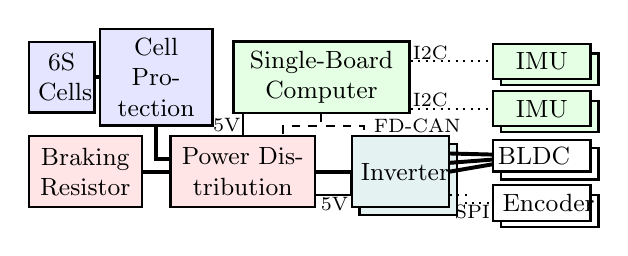
\begin{tikzpicture}[scale=1]   

    \node [rectangle, thick, draw, align=center, fill=blue!10, minimum height = 0.9cm, text width=0.6cm, font={\small}] (Cells) at (-1.5,1.2) 
    {6S Cells};

    \node [rectangle, thick, draw, align=center, fill=blue!10, minimum height = 0.9cm, text width=1.2cm, font={\small}] (BatteryProt) at (-0.3,1.2) 
    {Cell Protection};

    \node [rectangle, thick, draw, align=center, fill=red!10, minimum height = 0.9cm, text width=1.6cm, font={\small}] (PowerDistro) at (0.8,0)
    {Power Distribution};
    \node [rectangle, thick, draw, align=center, fill=red!10, minimum height = 0.9cm, text width=1.2cm, font={\small}] (BrakingResistor) at (-1.2,0)
    {Braking Resistor};
    
    \node [rectangle, thick, draw, align=center, fill=teal!10, minimum height = 0.9cm, text width=1cm, font={\small}] (InverterShadow) at (2.9,-0.1){};
    \node [rectangle, thick, draw, align=center, fill=teal!10, minimum height = 0.9cm, text width=1cm, font={\small}] (Inverter) at (2.8,0)
    {Inverter};

    \node [rectangle, thick, draw, align=center, fill=white, minimum height = 0.4cm, text width=1cm, align=center, font={\small}] (BLDCShadow) at (4.7,0.1)
    {};
    \node [rectangle, thick, draw, align=center, fill=white, minimum height = 0.4cm, text width=1cm, align=center, font={\small}] (BLDC) at (4.6,0.2)
    {};
    \node[align=center, font={\small}] at (4.5, 0.2) {BLDC};

    \node [rectangle, thick, draw, align=center, fill=white, minimum height = 0.4cm, text width=1cm, align=center, font={\small}] (EncoderShadow) at (4.7,-0.5)
    {};
    \node [rectangle, thick, draw, align=center, fill=white, minimum height = 0.4cm, text width=1cm, align=center, font={\small}] (Encoder) at (4.6,-0.4)
    {Encoder};

    \node [rectangle, thick, draw, align=center, fill=green!10, minimum height = 0.9cm, text width=2cm, font={\small}] (SBC) at (1.8,1.2)
    {Single-Board Computer};
    
    \node [rectangle, thick, draw, align=center, fill=green!10, minimum height = 0.4cm, text width=1cm, font={\small}] (IMU1Shadow) at (4.7,0.7)
    {};
    \node [rectangle, thick, draw, align=center, fill=green!10, minimum height = 0.4cm, text width=1cm, font={\small}] (IMU1) at (4.6,0.8)
    {IMU};
    
    \node [rectangle, thick, draw, align=center, fill=green!10, minimum height = 0.4cm, text width=1cm, font={\small}] (IMU2Shadow) at (4.7,1.3)
    {};
    \node [rectangle, thick, draw, align=center, fill=green!10, minimum height = 0.4cm, text width=1cm, font={\small}] (IMU2) at (4.6,1.4)
    {IMU};

    \begin{scope}[
        every node/.style={rectangle, align=center, font={\scriptsize}},
        every edge/.style={thick, draw, line width = 0.25mm},
        every path/.style={thick, draw, line width = 0.25mm}
    ]

        \draw[dotted] (SBC.east)++(0,-0.4) |- node [above right=-0.1cm]{I2C} (IMU1.west);
        \draw[dotted] (SBC.east)++(0,0.2)  |- node [above right=-0.1cm]{I2C} (IMU2.west);
        \draw[dotted] (Inverter.-25) -| ++(0.2,0) |- (Encoder.west) node [below left=-0.1cm]{SPI} ;
        \draw[-] (SBC.south)++(-1,0) -- node [left=-0.1cm]{5V} (PowerDistro.north);
        \draw[dashed] (SBC.south)++(0,0) -- ++(0,-0.15) -| node [right]{FD-CAN} (Inverter.135);
        \draw[dashed] (SBC.south)++(0,0) -- ++(0,-0.15) -| (PowerDistro.42);
        \draw[-] (PowerDistro.east)++(0,-0.3) -| node [below left=-0.1cm]{5V}  (Inverter.west);
    \end{scope}
    
    \begin{scope}[
        every node/.style={rectangle, align=center, font={\scriptsize}},
        every edge/.style={very thick, draw, line width = 0.5mm},
        every path/.style={very thick, draw, line width = 0.5mm}
    ]
        \draw[-] (Cells) -- (BatteryProt);
        \draw[-] (BatteryProt.south) |- (PowerDistro.170);
        \draw[-] (PowerDistro.west) -- (BrakingResistor.east);
        \draw[-] (PowerDistro) -- (Inverter);
        \draw[-] (Inverter.20) --  (BLDC);
        \draw[-] (Inverter.10)  --  (BLDC);
        \draw[-] (Inverter.0) -- (BLDC);
    \end{scope}

\end{tikzpicture}
